\section{Multilayer Perceptron}

Einee der bekanntesten Architekturen der neuronalen Netze ist das sogenannte \emph{Multilayer Perceptron}. Diese sehr vielfältig eingesetzte Struktur verwendet den erläuterten Backpropagation-Lernalgorithmus und erzielt damit in der Regel sehr gute Ergebnisse. Beim MLP spielt die Aktivierungsfunktion durchaus auch eine tragende Rolle und ist nicht fest definiert (häufig wird jedoch die Sigmoid-Funktion verwendet). Wenn das Netzwerk sehr viele verborgene Zwischenschichten besitzt wird es allgemein als \emph{tief} bezeichnet kann es zu Problemen beim Training kommen. Hierbei gibt es spezielle Techniken die dieses Problem lösen können und generell unter dem Namen \emph{depplearning} zusammengefasst werden. Da diese Architektur als so vielfältig gilt kann sie in vielen verschiedenen Anwendungsbereichen eingesetzt werden, hier ein paar Beispiele: 

\begin{multicols}{2}
\begin{itemize}
\item Mustererkennung 
\item Funktionenapproximation
\item Klassifizierung
\item Prognose,
\item Diagnose
\item Steuerung 
\item Optimierung
\end{itemize}
\end{multicols}

\begin{figure}[!htb]
	\centering
	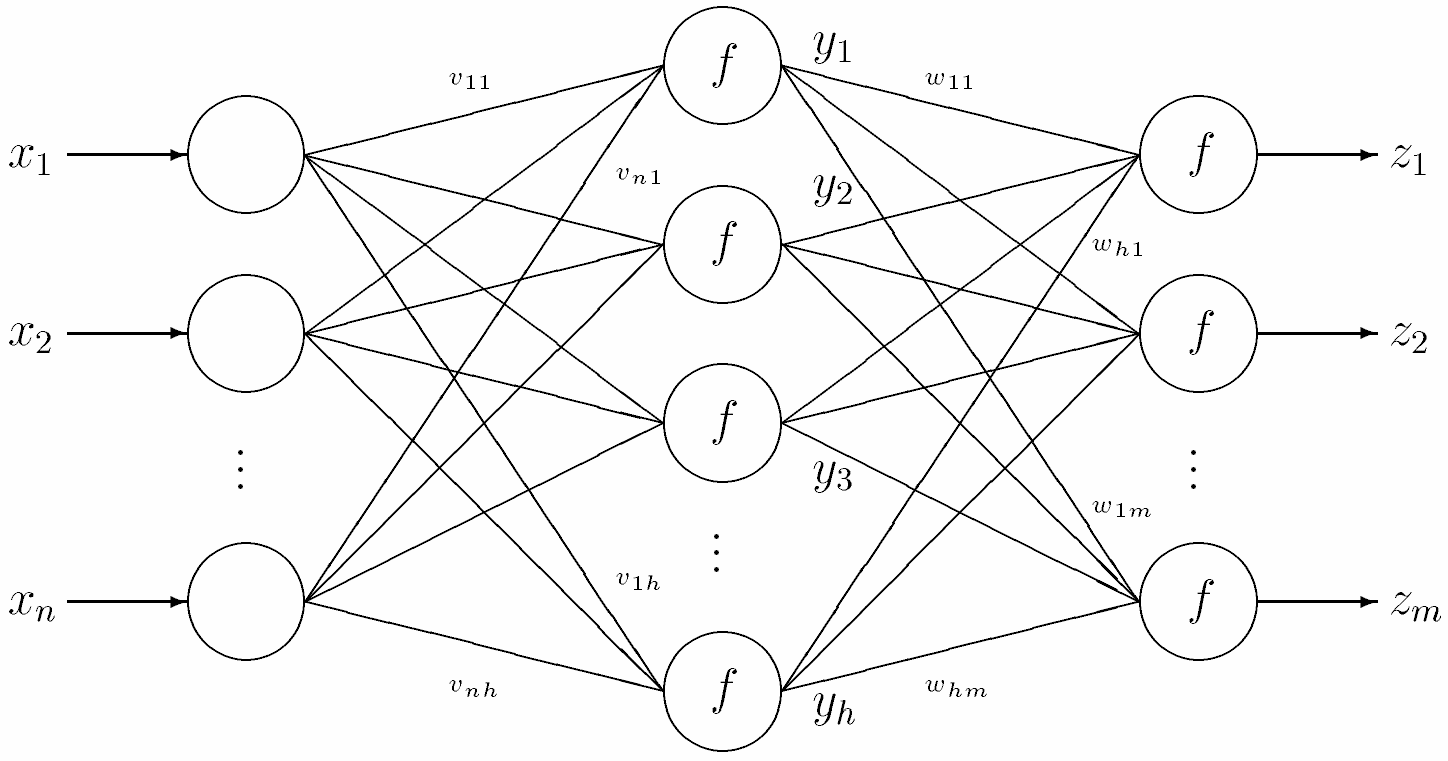
\includegraphics[width=.8\linewidth]{./img/mlp1}
	\mycaption{MLP - Aufbau}{ss}
	\label{fig:erstesPerceptron}
\end{figure}